%%%%%%%%%%%%%%%%%%%%%%%%%%%%%%%%%%%%%%%%%%%%%%%%%%%%%%%%%%%%%%%%%%%%%%%%%%%%%%%%
\chapter{Orbital Mechanics}
%%%%%%%%%%%%%%%%%%%%%%%%%%%%%%%%%%%%%%%%%%%%%%%%%%%%%%%%%%%%%%%%%%%%%%%%%%%%%%%%

Orbital mechanics \cite{Curtis2014} (a.k.a. ``astrodynamics'' \cite{Wakker2015}, ``celestial mechanics'' \cite{fitzpatrick_2012} or ``space dynamics'' \cite{thomson1986introduction}) is the study of the motion of objects in space. It is a branch of classical mechanics and is concerned with the motion of objects in the Solar System, and the motion of artificial satellites in orbit around bodies. It deals primarily with this through the application of ballistics, usually calculated through ``Newton's laws of motion'' and ``law of universal gravitation''. It is also concerned with the motion of spacecraft in interplanetary space, and the motion of spacecrafts in orbit around other planets.

This chapter deals with the relevant concepts of astrodynamics which adhere to standards of spaceflight engineering. It is not a comprehensive treatment of the subject, but rather a brief of the relevant topics which may arise in an asteroid mission. The chapter is divided into three sections: \autoref{sec:fundamentals_astrodynamics} deals with the basics of orbital mechanics, \autoref{sec:reference_frames} deals with reference frames and orbital elements, \autoref{sec:orbital_perturbations} deals with the basics of orbital perturbations and finally \autoref{sec:numerical_astrodynamics} deals with numerical methods for solving the equations of motion in astrodynamics.

%%%%%%%%%%%%%%%%%%%%%%%%%%%%%%%%%%%%%%%%%%%%%%%%%%%%%%%%%%%%%%%%%%%%%%%%%%%%%%%%
\section{Brief Fundamentals of Astrodynamics}\label{sec:fundamentals_astrodynamics}
%%%%%%%%%%%%%%%%%%%%%%%%%%%%%%%%%%%%%%%%%%%%%%%%%%%%%%%%%%%%%%%%%%%%%%%%%%%%%%%%

Newton's law of gravitation leads to the following nonlinear second-order differential equation which governs the motion of the body of mass $m_2$ around the body of mass $m_1$, which contains six vector constants of integration \cite[p.~67]{Curtis2014}:

\begin{equation}
    \ddot{\gls{om:r:vec}}=-\frac{\gls{om:mu}}{r^3}\gls{om:r:vec},
    \label{eq:newtons_equation_planetary}
\end{equation}
\begin{equation*}
    \begin{aligned}
        \textrm{where }
        \gls{om:r:vec} & =\textrm{the rectangular coordinate vector position relative to the central body,}         \\
        \gls{om:mu}        & =GM=G(m_1 + m_2)=\textrm{the gravitational parameter of the two-body system,}              \\
        \eqdesc{om:G}\text{ ,}                                                                                  \\
        m_1        & =\textrm{the mass of the primary (a.k.a. central) body, }                                  \\
        m_2        & =\textrm{the mass of the secondary body, often omitted from M when \ensuremath{m_1>>m_2}.} \\
    \end{aligned}
\end{equation*}

%%%%%%%%%%%%%%%%%%%%%%%%%%%%%%%%%%%%%%%%%%%%%%%%%%%%%%%%%%%%%%%%%%%%%%%%%%%%%%%%
\subsection{Two-body problem}\label{sec:two_body_problem}
%%%%%%%%%%%%%%%%%%%%%%%%%%%%%%%%%%%%%%%%%%%%%%%%%%%%%%%%%%%%%%%%%%%%%%%%%%%%%%%%

The \textbf{two-body (restricted) problem} is an analytical study whereby a secondary body with $m_2<<m_1$ has only a point mass gravitational acceleration acting on it due to the primary body's influence with mass $m_1$. The motion within the two-body system lies always within a plane (referred to as the centre of mass frame), owing also to the angular momentum vector is constant. Without non-conservative forces acting as perturbations, the energy of this system is constant, during the exchange of kinetic into potential energy leading up to the apoapsis and vice versa at the periapsis (respectively the largest and smallest instances of separation).

\begin{figure}
    \centering
    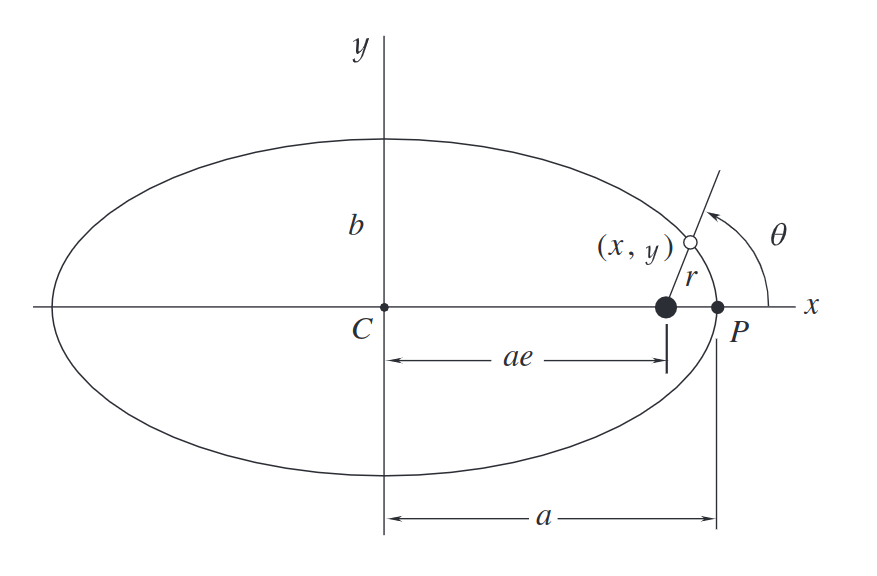
\includegraphics[width=0.6\linewidth]{graphics/orbit.png}
    \captionsetup{format=hang} % hanging captions
    \caption{\textbf{Elliptical orbit of a two-body system.} The orbit of a two-body system is an ellipse when $e\in(0,1)$, with the periapsis and apoapsis being the closest and farthest points of separation, respectively. The orbit is always contained within a plane, and the angular momentum vector is constant. Figure taken from Curtis \cite[p.~88]{Curtis2014}.}
    \label{fig:orbit}
\end{figure}

The governing analytical solution of the two-body problem is referred to as the ``orbit equation'' can be derived to be \cite[p.~77]{Curtis2014}:

\begin{equation}
    r=\gls{fn:fn}(\nu)=\frac{h^2}{\gls{om:mu}}\frac{1}{1+e\cos\nu},
    \label{eq:orbit_equation}
\end{equation}
\begin{equation*}
    \begin{aligned}
        \textrm{where }
        h   & =\textrm{the specific angular momentum secondary body's orbit,} \\
        e   & =\textrm{the eccentricity of orbit,}                            \\
        \nu & =\textrm{the true anomaly of secondary body.}                   \\
    \end{aligned}
\end{equation*}

%%%%%%%%%%%%%%%%%%%%%%%%%%%%%%%%%%%%%%%%%%%%%%%%%%%%%%%%%%%%%%%%%%%%%%%%%%%%%%%%
\newpage\section{Reference Frames}\label{sec:reference_frames}
%%%%%%%%%%%%%%%%%%%%%%%%%%%%%%%%%%%%%%%%%%%%%%%%%%%%%%%%%%%%%%%%%%%%%%%%%%%%%%%%

A \textbf{reference frame} (a.k.a. ``frame'') is defined by an ordered set of three mutually orthogonal, possibly time-dependent, unit-length direction vectors and a \textbf{coordinate system} specifies a mechanism for locating points within a frame. \cite[p.~4]{SpiceReferenceFrames2020}. There are various categories of frames used within astrophysics and astrodynamics. Some frames are outdated in nature but are however still documented and commonly used to ensure the usability of historical empirical data. Some coordinate systems are standardised, however, many are not and therefore data users and producers must remain attentive. This section will cover the generalised taxonomy of these frames, with a mention of common frames and where they fit within the taxonomy.

\begin{figure}[h]
    \centering
    \def\svgwidth{0.72\linewidth}
    \captionsetup{format=hang} % hanging captions
    \import{graphics/}{ths_base_frame.pdf_tex}
    \caption{\textbf{Right-handed reference frame.} The right-handed ($\mathbf{X}\cross{\mathbf{Y}}=\mathbf{Z}$) frame is defined by the three mutually orthogonal unit vectors $\mathbf{i}$, $\mathbf{j}$ and $\mathbf{k}$, which are respectively the $x$, $y$ and $z$ axes. }
    \label{fig:frames_rh}
\end{figure}

Unless stated otherwise, one should assume that all frames used within astrodynamics are right-handed, defined by $\mathbf{X}\cross{\mathbf{Y}}=\mathbf{Z}$ as illustrated in \autoref{fig:frames_rh}. The contemporary reference systems used in astronomy and astrophysics are often defined by the \gls{IAU}. Due to the long history of the field, there are many others outside of the \glsposs{IAU} standardised frames which are still used for a multitude of reasons, one being the need to ensure accessibility to older observations and processed data which were made in the outdated systems.

%%%%%%%%%%%%%%%%%%%%%%%%%%%%%%%%%%%%%%%%%%%%%%%%%%%%%%%%%%%%%%%%%%%%%%%%%%%%%%%%
\subsection{Inertial}\label{ssec:frame_intertial}
%%%%%%%%%%%%%%%%%%%%%%%%%%%%%%%%%%%%%%%%%%%%%%%%%%%%%%%%%%%%%%%%%%%%%%%%%%%%%%%%

An inertial reference frame is a non-rotating (with respect to the stars) frame with a non-accelerating origin. All inertial frames remain in a state of mutual constant rectilinear motion with respect to one another.  There are two frames which are used in astrophysics at the lowest level in the hierarchy, namely J2000 (a.k.a. EME 2000) and the \gls{ICRF}. The current standard is to opt for the use of the ICRF, however, for many applications, the use of one over the other is negligible, as the ICRF was defined to coincide almost precisely with the J2000 frame (differing by $<0.1$ arc second $\approx 2.8\times 10^{-5}$ degrees). The ICRF frame is defined through observations made with \gls{VLBI}, with its axes defined such that it shows ``no global rotation with respect to a set of distant extragalactic objects''  \cite{IAU1991, IAU1997}. The number of distant extragalactic radio sources used in the definition of the frame is 295. Finally, the origin of the frame is defined to be the barycenter of the Solar System as seen in \autoref{fig:icrf_frame}.

\begin{figure}
    \centering
    \captionsetup{format=hang} % hanging captions
    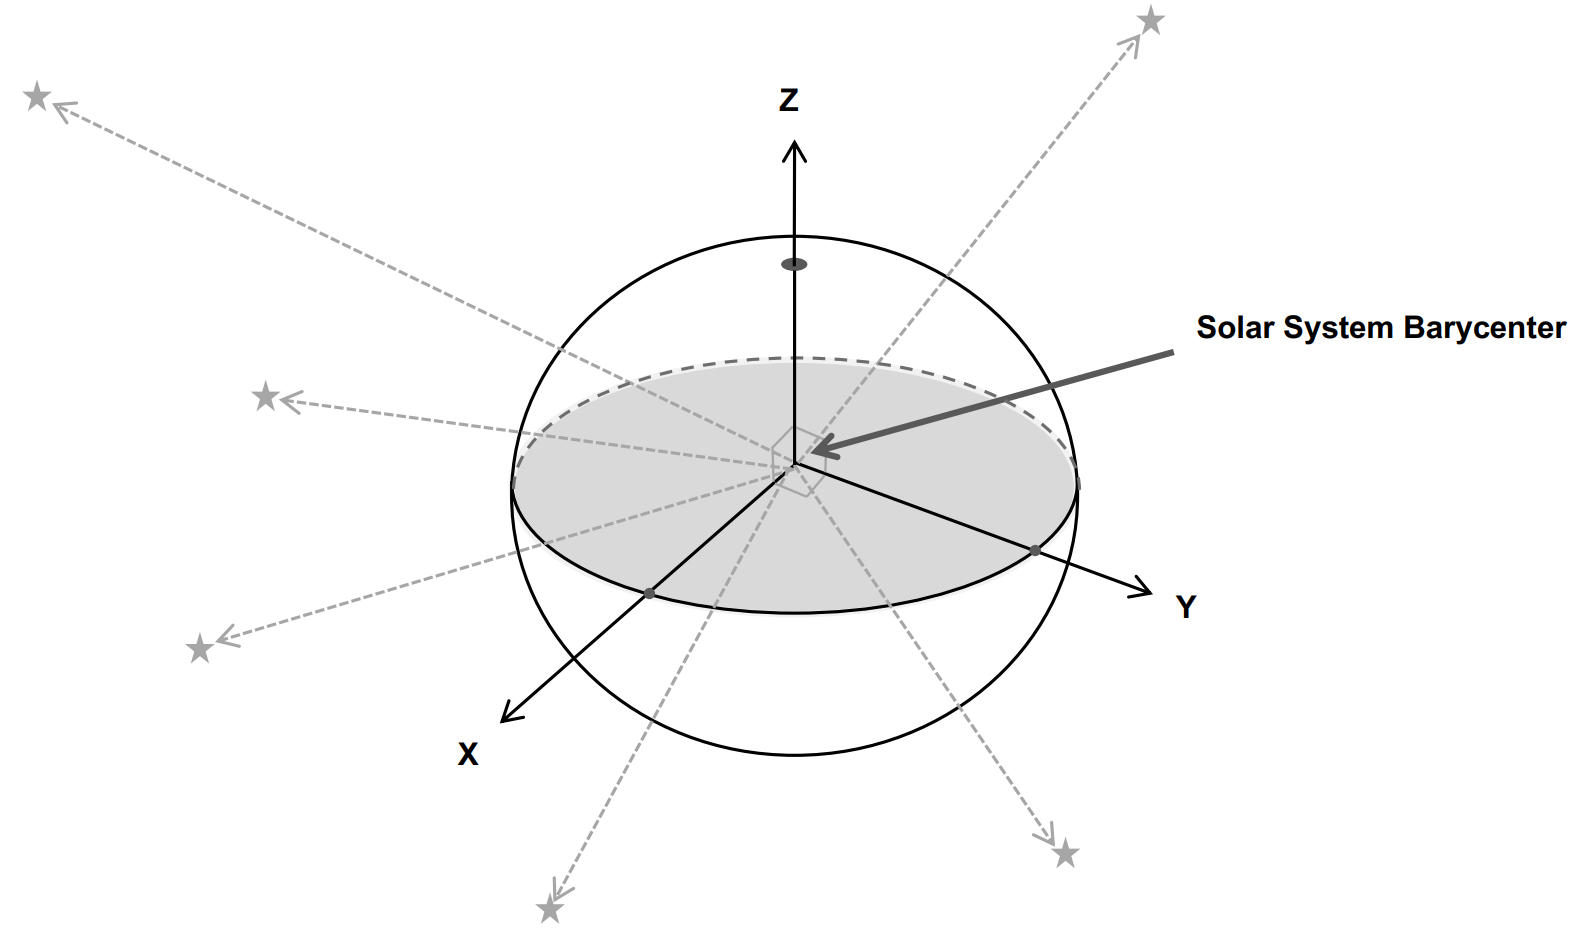
\includegraphics[width=0.72\linewidth]{graphics/icrf.png}
    \caption{\textbf{International Celestial Reference Frame (ICRF)}. The \gls{ICRF} is defined by 295 extragalactic radio sources with its centre situated at the barycentre of the Solar System. Figure retrieved from \gls{NAIF} SPICE tutorials on reference frames \cite[p.~11]{SpiceReferenceFrames2020}}
    \label{fig:icrf_frame}
\end{figure}

%%%%%%%%%%%%%%%%%%%%%%%%%%%%%%%%%%%%%%%%%%%%%%%%%%%%%%%%%%%%%%%%%%%%%%%%%%%%%%%%
\subsection{Body-centered inertial (BCI)}
%%%%%%%%%%%%%%%%%%%%%%%%%%%%%%%%%%%%%%%%%%%%%%%%%%%%%%%%%%%%%%%%%%%%%%%%%%%%%%%%

A \Gls{BCI} frame is non-rotating with respect to the stars. It can be derived from the \gls{ICRF} or J2000 mentioned in \autoref{ssec:frame_intertial} with the only difference being the offset of the origin to the centre of mass of a body and often a rotation to align the $Z$ axis with the rotational axis of the body. Strictly speaking, this origin is accelerating towards the barycentre of the Solar System, however, the impact of the accelerating origin of a major celestial planet can be ignored on accuracy is considered negligible allowing for the application of Newton's laws and special relativity. Due to this small caveat, these frames are sometimes referred to as ``quasi-inertial'' frames. In the case of the \gls{ECI}, the $Z$-axis is directed along the (counterclockwise positive) spin-axis of the body, and the $X$-axis passes through the ascending node of the intersection between the ecliptic and the equator of the body. The $Y$-axis then passes through the equatorial plane perpendicular to the $X$ and $Z$-axis to complete the frame. The \gls{ECI} is often used to describe the motion of objects within the Earth's sphere of influence. The \gls{ECI} frame illustrated in \autoref{fig:ECI}.

\begin{figure}[H]
    \centering
    \def\svgwidth{0.72\linewidth}
    % \input{graphics/drawing2.pdf_tex}
    \import{graphics/}{ths_j2000.pdf_tex}
    \caption{Definition of the J2000 Earth-centred inertial (ECI) frame.}
    \label{fig:ECI}
\end{figure}

%%%%%%%%%%%%%%%%%%%%%%%%%%%%%%%%%%%%%%%%%%%%%%%%%%%%%%%%%%%%%%%%%%%%%%%%%%%%%%%%
\subsection{Body-centered body-fixed (BCBF)\label{ssec:frame_bcbf}}
%%%%%%%%%%%%%%%%%%%%%%%%%%%%%%%%%%%%%%%%%%%%%%%%%%%%%%%%%%%%%%%%%%%%%%%%%%%%%%%%

The body-centred body-fixed (BCBF) reference frames are frames which have their origins at the centre of mass of a body, the $Z_F$-axis is directed along the (counter clockwise positive) spin-axis of the body. The $X_F$-axis passes through the reference meridian of the body, which is at an angle of $\Omega_t{t_0}$ from the ascending node of the intersection between the ecliptic and the equator of the body. The $Y_F$-axis then passes through the equatorial plane perpendicular to $X_F$ and $Z_F$.

\begin{figure}[H]
    \centering
    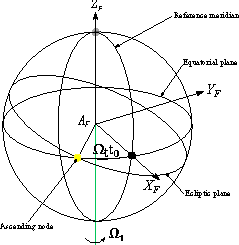
\includegraphics[width=0.35\linewidth]{graphics/bcbf.pdf}
    \caption{
        Definition of a general Body-centered body-fixed (BCBF) reference frame.
    }
    \label{fig:bci}
\end{figure}


\begin{equation}
    W = W_0 + \dot{W}d
    \label{eq:ephem_prime_meridian}
\end{equation}
\begin{equation*}
    \begin{aligned}
        \textrm{where, }
        W   & = \textrm{the ephemeris position of the prime meridian}               \\
        W_0 & = \textrm{the value of W at J2000.0 (occasionally some other epoch),} \\
        d   & = \textrm{interval in days from the standard epoch.}
    \end{aligned}
\end{equation*}

\begin{equation}
    \mathbf{R}^{I/B}=\mathbf{R}_z(W)\mathbf{R}_x(\pi/2-\delta_0)\mathbf{R}_z(\pi/2-\alpha_0)
    \label{eq:bci_transformation}
\end{equation}
\begin{equation*}
    \begin{aligned}
        \textrm{where, }
        \mathbf{R}_{x,y,z}(\phi) & = \textrm{transformation matrix for a rotation of $\phi$ radians about the respective axis (\autoref{appendix:rotational_transformations}),} \\
        \alpha_0, \delta_0       & = \textrm{ICRF equatorial coordinates at epoch J2000.0}                                                                                      \\
    \end{aligned}
\end{equation*}

% %%%%%%%%%%%%%%%%%%%%%%%%%%%%%%%%%%%%%%%%%%%%%%%%%%%%%%%%%%%%%%%%%%%%%%%%%%%%%%%%
% \subsection{Radial tangential normal (RTN)\label{ssec:frame_rtn}\label{ssec:frame_rsw}}
% %%%%%%%%%%%%%%%%%%%%%%%%%%%%%%%%%%%%%%%%%%%%%%%%%%%%%%%%%%%%%%%%%%%%%%%%%%%%%%%%

% The radial tangential normal frame (RTN), a.k.a. the radial (R), along-track (S) and cross-track (W) frame (RSW), is a dynamic frame with an orbiting spacecraft at the centre of the frame. The frame is time-dependent and based on the two-body restricted problem with the R-component determined by the current unit-vector of position $\hat{r}$, the T-component by the unit vector of velocity $\hat{v}$, and the N-component by their cross product of the two, the specific angular momentum vector $\hat{r}\cross{\hat{v}}=\hat{h}$. This frame is commonly used for the relative motion of spacecraft in a rendezvous segment.

% \begin{equation}
%     \mathbf{R}^{I/RSW}= \bigg[\hat{\gls{om:r:vec}}_{B/S}\; \hat{\gls{om:v:vec}}_{B/S}\; \hat{\mathbf{h}}_{B/S} \bigg]
% \end{equation}
% \begin{equation*}
%     \begin{aligned}
%         \textrm{where, }
%         \hat{\gls{om:r:vec}}_{B/S} &= \textrm{the position of the spacecraft with respect to the body,}\\
%         \hat{\gls{om:v:vec}}_{B/S} &= \textrm{the velocity of the spacecraft with respect to the body,}\\
%         \hat{\mathbf{h}}_{B/S} &= \textrm{the specific angular momentum of the spacecraft with respect to the body,}\\
%     \end{aligned}
% \end{equation*}

%%%%%%%%%%%%%%%%%%%%%%%%%%%%%%%%%%%%%%%%%%%%%%%%%%%%%%%%%%%%%%%%%%%%%%%%%%%%%%%%
\newpage\subsection{Relative Orbital (RSW)\label{ssec:relative_orbital_frame}}
%%%%%%%%%%%%%%%%%%%%%%%%%%%%%%%%%%%%%%%%%%%%%%%%%%%%%%%%%%%%%%%%%%%%%%%%%%%%%%%%

% See \cite[p.~159]{Vallado2013} for a detailed description of all reference frames.

The relative orbital frame is a dynamic frame with spacecraft A at the centre of the frame on the ``target orbit'' or ``reference orbit''. The frame is time-dependent (corotating) with the $X$-axis determined by the current inertial unit-vector of position $\gls{om:r:vec}_A$, the $Z$-axis by the unit vector of the specific angular momentum vector $\mathbf{h}_A=\gls{om:r:vec}_A\cross{\gls{om:v:vec}_A}$, and the $Y$-axis by their cross product. This frame is commonly used for the relative motion of spacecraft in a rendezvous segment.

\begin{figure}[H]
    \centering
    \captionsetup{format=hang} % hanging captions
    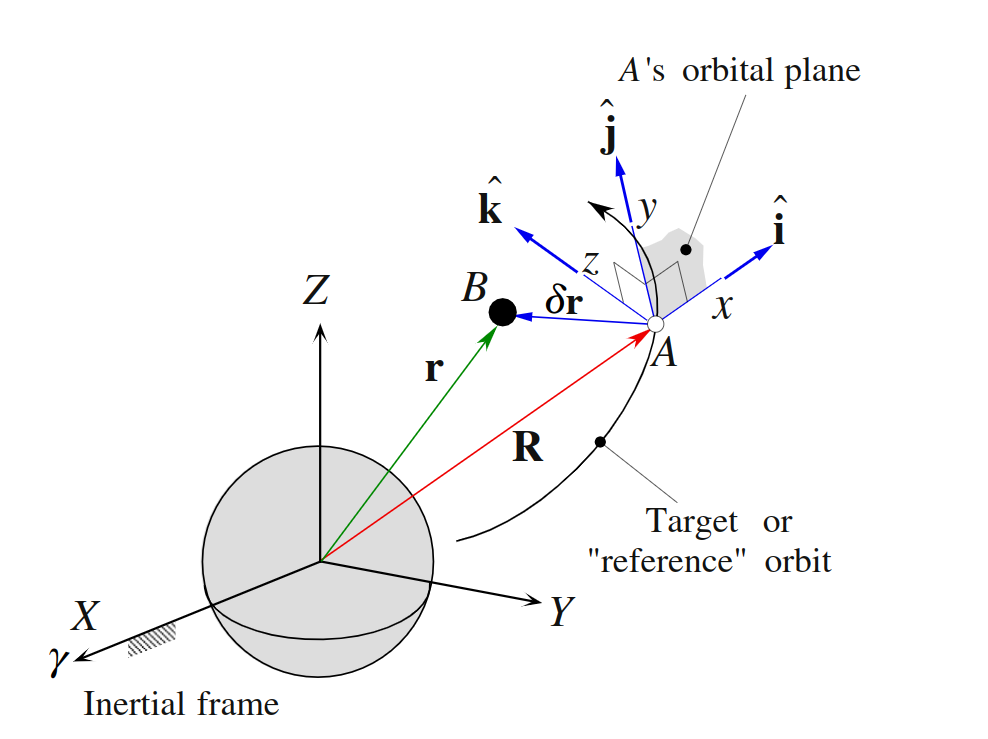
\includegraphics[width=0.6\linewidth]{graphics/relative_frame.png}
    \caption{\textbf{Relative Orbital Motion Frame}. A reference orbit is defined by spacecraft A. Spacecraft B is in an observed orbit. The relative orbital frame is defined by the position and velocity of spacecraft A. This corotating non-inertial frame is referred to as the LVLH (local-vertical-local-horizontal) frame of A. Figure retrieved from Curtis \cite[p.~368]{Curtis2014}}
    \label{fig:relative_orbital_frame}
\end{figure}

Note that notation is adopted from Curtis \cite[p.~368]{Curtis2014}, however, the local spacecraft frame is equivalent to the RSW frame of A. The conversion process from an inertial reference frame centred on the primary (central) attracting body to the relative orbital frame is covered here, and taken from Curtis \cite[p.~368]{Curtis2014}. The following equations are used to define the orthogonal basis vectors of the relative orbital reference frame and are the first steps in determining relative motion in the dynamic frame:

\begin{subequations}
    \begin{align}
        \begin{split}\hat{\mathbf{i}}&=\frac{\gls{om:r:vec}_A}{r_A}\end{split} \\
        \begin{split}\hat{\mathbf{j}}&=\frac{\mathbf{h}_A}{h_A}\end{split} \\
        \begin{split}\hat{\mathbf{k}}&=\hat{\mathbf{k}}\cross{\hat{\mathbf{i}}}.\end{split}
    \end{align}
    \label{eq:rel_frame}
\end{subequations}

The orthogonal transformation matrix $[\mathbf{Q}]_{X/x}$ from the inertial, body-centered reference frame $XYZ$ into the relative orbital frame $xyz$ (See \autoref{fig:relative_orbital_frame}) can then be calculated using the results of \autoref{eq:rel_frame}:

\begin{equation}
    [\mathbf{Q}]_{x/X}=\left[\begin{array}{ccc}l_x & m_x & n_x \\ l_y & m_y & n_y \\ l_z & m_z & n_z\end{array}\right] \quad \begin{aligned}&\leftarrow \text { components of } \hat{\mathbf{i}} \\&\leftarrow \text { components of } \hat{\mathbf{j}} \\&\leftarrow \text { components of } \hat{\mathbf{k}}\end{aligned}
    \label{eq:relative_frame_transformation}
\end{equation}

The angular velocity of the relative orbital frame is then given by is calculated using the following equation:

\begin{equation}
    \boldsymbol{\Omega}=\frac{\mathbf{h}_A}{h_A^2}= \frac{\gls{om:r:vec}_A\cross{\gls{om:v:vec}_A}}{r_A},
\end{equation}

followed by the angular acceleration of the relative orbital frame using the following equation:

\begin{equation}
    \dot{\boldsymbol{\Omega}}=-2\frac{\gls{om:v:vec}_A{\cdot}\gls{om:r:vec}_A}{r_A^4}\mathbf{h}_A=-2\frac{\gls{om:v:vec}_A{\cdot}\gls{om:r:vec}_A}{r_A^2}\boldsymbol{\Omega}.
\end{equation}

The relative position, velocity and acceleration in the \textbf{inertial} reference frame are calculated using the following equations:

\begin{subequations}
    \begin{align}
        \begin{split}\gls{om:r:vec}_{\mathrm{rel}} &=\gls{om:r:vec}_B-\gls{om:r:vec}_A \end{split}                                                      \\
        \begin{split}\gls{om:v:vec}_{\mathrm{rel}} &=\gls{om:v:vec}_B-\gls{om:v:vec}_A-\boldsymbol{\Omega} \times \gls{om:r:vec}_{\mathrm{rel}} \end{split} \\
        \begin{split}\mathbf{a}_{\mathrm{rel}} &=\mathbf{a}_B-\mathbf{a}_A-\dot{\boldsymbol{\Omega}} \times \gls{om:r:vec}_{\mathrm{rel}}-\boldsymbol{\Omega} \times\left(\boldsymbol{\Omega} \times \gls{om:r:vec}_{\mathrm{rel}}\right)-2 \boldsymbol{\Omega} \times \gls{om:v:vec}_{\mathrm{rel}}\end{split}
    \end{align}
    \label{eq:relative_inertial_frame}
\end{subequations}

Using the transformation in \autoref{eq:relative_frame_transformation}, and the results of \autoref{eq:relative_inertial_frame} the relative position, velocity and acceleration in the \textbf{relative orbital} reference frame are calculated using the following equations:

\begin{subequations}
    \begin{align}
        \begin{split}\left\{\gls{om:r:vec}_{\text{rel}}\right\}_x &=[\mathbf{Q}]_{x/X}\left\{\gls{om:r:vec}_{\text{rel}}\right\}_X\end{split} \\
        \begin{split}\left\{\gls{om:v:vec}_{\text{rel}}\right\}_x &=[\mathbf{Q}]_{x/X}\left\{\gls{om:v:vec}_{\text{rel}}\right\}_X\end{split} \\
        \begin{split}\left\{\mathbf{a}_{\text{rel}}\right\}_x &=[\mathbf{Q}]_{x/X}\left\{\mathbf{a}_{\text{rel}}\right\}_X\end{split}
    \end{align}
\end{subequations}

With the performed steps, the relative position, velocity and acceleration in the \textbf{relative orbital} reference frame are now known. It is often that approximations of these equations are further derived, one of which is the well-known ``Clohessy Wiltshire'' equations \cite{CLOHESSY2012}, which assumes the target orbit is circular. An alternative linear second-order approximation is given here. Let the inertial positions of A (reference orbit) and B (observed orbit), $\gls{om:r:vec}_A$ and $\gls{om:r:vec}_B$ be denoted now as $\mathbf{R}$ and $\gls{om:r:vec}$ respectively. The relative position of the observed orbit relative to the reference orbit is denoted as $\delta \gls{om:r:vec}$ resulting in:

\begin{equation}
    \gls{om:r:vec}=\mathbf{R}+\delta \gls{om:r:vec}
\end{equation}

The linear second-order equations of motions derived by Curtis \cite[p.~380]{Curtis2014} assumes that the relative position is small compared to the position of A $(\delta r / R << 1)$, resulting in the expression:

\begin{subequations}
    \begin{align}
        \begin{split} &\delta \ddot{x}-\left(\frac{2 \gls{om:mu}}{R^3}+\frac{h^2}{R^4}\right) \delta x+\frac{2(\mathbf{V} \cdot \mathbf{R}) h}{R^4} \delta y-2 \frac{h}{R^2} \delta \dot{y}=0 \end{split} \\
        \begin{split} &\delta \ddot{y}+\left(\frac{\gls{om:mu}}{R^3}-\frac{h^2}{R^4}\right) \delta y-\frac{2(\mathbf{V} \cdot \mathbf{R}) h}{R^4} \delta x+2 \frac{h}{R^2} \delta \dot{x}=0 \end{split}   \\
        \begin{split} &\delta \ddot{z}+\frac{\gls{om:mu}}{R^3} \delta z=0\end{split}
    \end{align}
\end{subequations}

Alternative parametrisations have been proposed such as the use of nodal elements \cite{Leomanni2020} and a Hamiltonian approach including perturbations \cite{Kolemen2005}.

%%%%%%%%%%%%%%%%%%%%%%%%%%%%%%%%%%%%%%%%%%%%%%%%%%%%%%%%%%%%%%%%%%%%%%%%%%%%%%%%
\newpage\section{Orbital Elements}
%%%%%%%%%%%%%%%%%%%%%%%%%%%%%%%%%%%%%%%%%%%%%%%%%%%%%%%%%%%%%%%%%%%%%%%%%%%%%%%%
Due to their thorough use throughout different standards of numerical simulation and navigational data formats, this section is dedicated to listing the most common orbital elements and their definitions. The orbital elements are defined as the six independent parameters that are required to fully describe the orbit of a body in space around a primary body in the absence of any external perturbations incurred in the system. When using the term ``Elements``, we are generally describing the motion of a body with negligible mass in comparison to its primary gravitational attractor. For example, one would not generally describe the state of a Lunar orbiter in an orbit around Earth as the intuition gained by using orbital elements resides within the context of the restricted two-body problem. Orbital elements are canonically defined with respect to an inertial plane of reference and reference direction. Conversion between any arbitrary pair of orbital elements of a given reference plane and direction requires only the central body's gravitational parameter $\gls{om:mu}$.

\autoref{ssec:cartesian} covers the cartesian orbital elements representation, which encapsulates the Cartesian coordinates of the spacecraft in its instantaneous orbital state, \autoref{ssec:keplerian} describes the Keplerian elements (a.k.a. ``classical orbital elements'') and finally, the modified equinoctial elements are discussed in \autoref{ssec:equinoctial}.

%%%%%%%%%%%%%%%%%%%%%%%%%%%%%%%%%%%%%%%%%%%%%%%%%%%%%%%%%%%%%%%%%%%%%%%%%%%%%%%%
\subsection{Cartesian}\label{ssec:cartesian}
%%%%%%%%%%%%%%%%%%%%%%%%%%%%%%%%%%%%%%%%%%%%%%%%%%%%%%%%%%%%%%%%%%%%%%%%%%%%%%%%
The Cartesian, a.k.a. the rectangular orbital elements are the concatenation of
the position and velocity vectors in the respectively named coordinate system
relative to the central body,

\begin{equation}
    \gls{om:oe:cartesian}=
    \{
    \myvec{r},
    \myvec{v}
    \}
    =
    \{
    r_x,
    r_y,
    r_z,
    v_x,
    v_y,
    v_z
    \}
\end{equation}

where all values are assumed as S.I. units, where not specified otherwise, in
further calculations involving the orbital elements.

%%%%%%%%%%%%%%%%%%%%%%%%%%%%%%%%%%%%%%%%%%%%%%%%%%%%%%%%%%%%%%%%%%%%%%%%%%%%%%%%
\subsection{Keplerian}\label{ssec:keplerian}
%%%%%%%%%%%%%%%%%%%%%%%%%%%%%%%%%%%%%%%%%%%%%%%%%%%%%%%%%%%%%%%%%%%%%%%%%%%%%%%%
The Keplerian (a.k.a. the \textbf{classical orbital elements}, \textbf{two-body elements} or \textbf{osculating elements}) are a set of 6 quantities which define the state of a spacecraft in space using the description of the two-body restricted problem discussed in \autoref{sec:two_body_problem}. These elements are illustrated in \autoref{fig:keplerian_elements} and are defined as follows:

\begin{equation}
    \gls{om:oe:keplerian}= \{
    \gls{om:a},
    \gls{om:e},
    \gls{om:i},
    \gls{om:raan},
    \gls{om:argp},
    \gls{om:nu}
    \}
\end{equation}
\begin{equation*}
    \begin{aligned}
        \text{where, }
        \gls{om:a}    & = \text{Semi-major axis}                       \\
        \gls{om:e}    & = \text{Eccentricity}                          \\
        \gls{om:i}    & = \text{Inclination}                           \\
        \gls{om:raan} & = \text{Right ascension of the ascending node} \\
        \gls{om:argp} & = \text{Argument of periapsis}                 \\
        \gls{om:nu}   & = \text{True anomaly}
    \end{aligned}
\end{equation*}

\begin{figure}
    \centering
    \def\svgwidth{0.65\linewidth}
    \import{graphics/}{Orbit1.pdf_tex}
    \captionsetup{format=hang} % hanging captions
    \caption{\textbf{Keplerian orbital elements}. The six classical element
        quantities that define the state of a spacecraft in space are the semi-major axis $a$, the eccentricity $e$, the inclination $i$, the right ascension of the ascending node $\Omega$, the argument of periapsis $\omega$ and the true anomaly $\nu$. All quantities are illustrated, except for $e$ and $a$ which are illustrated in an elliptical orbit in \autoref{fig:orbit}.}
    \label{fig:keplerian_elements}
\end{figure}

Preliminary quantities required for the calculation of the classical orbital elements are the angular momentum vector $\mathbf{h}$, the eccentricity vector $\mathbf{e}$, the node vector $\mathbf{n}$ and the specific mechanical energy $\mathcal{E}$, which are calculated as follows:

\begin{subequations}
    \begin{alignat}{2}
        \mathbf{h}  & =\gls{om:r:vec} \times \gls{om:v:vec}                                       &  & \rightarrow\text{ angular momentum vector}    \\
        \mathbf{e}  & =\frac{\gls{om:v:vec} \times \mathbf{h}}{\gls{om:mu}}-\frac{\gls{om:r:vec}}{r}      &  & \rightarrow\text{ eccentricity vector}        \\
        \mathbf{n}  & =[0,0,1]^{\mathrm{T}} \times \mathbf{h}=[-h_y, h_x, 0]^{\mathrm{T}} &  & \rightarrow\text{ node vector}                \\
        \mathcal{E} & = \frac{v^2}{2}-\frac{\gls{om:mu}}{r}                                       &  & \rightarrow\text{ specific mechanical energy}
    \end{alignat}
\end{subequations}

The equations used in calculating the quantities in \gls{om:oe:keplerian} are taken from Vallado \cite[p.~95]{Vallado2013}. Quantities exhibiting an underline are intermediate values, for example, $\underline{\Omega}$ is used as an intermediate value to calculate $\Omega$ where a check determines its final value. These equations are:

\begin{subequations}
    \begin{align}
        \begin{split} a &= \begin{cases}-\frac{\gls{om:mu}}{2 \mathcal{E}} & \text{ for } e \neq 1 \\
             \infty                     & \text{ for } e = 1
            \end{cases} \end{split}                                                              \\
        \begin{split} p &= \begin{cases} a\left(1-e^2\right) & \text{ for } e \neq 1 \\
              \frac{h^2}{\gls{om:mu}}     & \text{ for } e = 1
            \end{cases} \end{split}                                                              \\
        \begin{split} i=\arccos \frac{h_y}{h} \end{split}                                                                      \\
        \begin{split} \underline{\Omega}=\arccos \frac{n_x}{n} \end{split}                                                     \\
        \begin{split} \underline{\omega}=\arccos \frac{\myvec{n} \cdot \myvec{e}}{n e} \end{split} \\
        \begin{split} \underline{\nu}=\arccos \frac{\myvec{e} \cdot \myvec{r}}{e r}\end{split}
    \end{align}
    \label{eq:cartesian_to_keplerian}
\end{subequations}

The final checks are then applied to the quantities of $\underline{\Omega}$, $\underline{\omega}$ and $\underline{\nu}$ to determine their final values. The checks are as follows:

\begin{subequations}
    \begin{align}
        \begin{split} \Omega &=
            \begin{cases}
                \underline{\Omega}        & \text{ for }  n_y \geq 0 \\
                2\pi - \underline{\Omega} & \text{ otherwise. }
            \end{cases}
        \end{split} \\
        \begin{split} \omega &=
            \begin{cases}
                \underline{\omega}        & \text{ for } e_z \geq 0 \\
                2\pi - \underline{\omega} & \text{ otherwise. }
            \end{cases}
        \end{split} \\
        \begin{split} \nu &=
            \begin{cases}
                \underline{\nu}         & \text{ for } {\myvec{r}} \cdot {\myvec{v}} \geq 0 \\
                2 \pi - \underline{\nu} & \text{ otherwise. }
            \end{cases}
        \end{split}
    \end{align}
    \label{eq:cartesian_to_keplerian_checks}
\end{subequations}

Note that if the orbit is parabolic ($\gls{om:e}=1$), $\gls{om:a}=\infty$, in which case the value of the semi-latus rectum $\gls{om:p}$ is used in its place to describe the orbit, as suggested by \autoref{eq:cartesian_to_keplerian}. Additionally, the mean anomaly $\gls{om:M}$ or time since periapsis passage $\gls{om:tp}$ can be used in the place of $\gls{om:nu}$. The conversion from classical orbital elements to cartesian can be found in Vallado \cite[p.~116]{Vallado2013}. The advantage of this state representation is the intuition gained in the orbital configuration, evident by \autoref{fig:keplerian_elements}, as only one parameter is time-varying in the restricted two-body problem. The disadvantages of using these elements are the singularities that occur in differential equations for $\gls{om:e}=0$ and $\gls{om:i}\in \{0,\pi/2\}$, seen in \autoref{eq:vop:gauss:kep}.

%%%%%%%%%%%%%%%%%%%%%%%%%%%%%%%%%%%%%%%%%%%%%%%%%%%%%%%%%%%%%%%%%%%%%%%%%%%%%%%%
\subsection{Modified Equinoctial}\label{ssec:equinoctial}
%%%%%%%%%%%%%%%%%%%%%%%%%%%%%%%%%%%%%%%%%%%%%%%%%%%%%%%%%%%%%%%%%%%%%%%%%%%%%%%%
The Modified Equinoctial Orbital elements are a set of orbital elements derived from the classical orbital elements. They are particularly useful in trajectory optimisation and analysis as they address the singularities in the classical elements for $\gls{om:e}=0$ and $\gls{om:i}\in \{0,\pi/2\}$.The modified equinoctial elements are defined as:

\begin{equation}
    \gls{om:oe:equinoctial}=
    \{
    p,
    f,
    g,
    h,
    k,
    L
    \}
\end{equation}

The equations for converting from the classical orbital elements in \autoref{ssec:keplerian} to the modified equinoctial elements are given by \cite{EquinoctalElements}:

\begin{subequations}
    \begin{alignat}{1}
        p= & a(1-e^2)                \\
        f= & e\cos{(\omega+\Omega)}  \\
        g= & e\cos{(\omega+\Omega)}  \\
        h= & \tan{(i/2)}\cos{\Omega} \\
        k= & \tan{(i/2)}\sin{\Omega} \\
        L= & \Omega+\omega+\nu       \\
    \end{alignat}
\end{subequations}

Note however the singularities for Keplerian orbits state in \autoref{ssec:keplerian} are replaced by singularities in the modified equinoctial elements for two elements at an orbital inclination of $\gls{om:i}=2\pi$. However, this orbital configuration is fully retrograde, and not generally desired due to increased orbit decay.

%%%%%%%%%%%%%%%%%%%%%%%%%%%%%%%%%%%%%%%%%%%%%%%%%%%%%%%%%%%%%%%%%%%%%%%%%%%%%%%%
% \section{Preliminary Orbit Determination}
% %%%%%%%%%%%%%%%%%%%%%%%%%%%%%%%%%%%%%%%%%%%%%%%%%%%%%%%%%%%%%%%%%%%%%%%%%%%%%%%%

% %%%%%%%%%%%%%%%%%%%%%%%%%%%%%%%%%%%%%%%%%%%%%%%%%%%%%%%%%%%%%%%%%%%%%%%%%%%%%%%%
% \subsection{Gibbs method}
% %%%%%%%%%%%%%%%%%%%%%%%%%%%%%%%%%%%%%%%%%%%%%%%%%%%%%%%%%%%%%%%%%%%%%%%%%%%%%%%%

% %%%%%%%%%%%%%%%%%%%%%%%%%%%%%%%%%%%%%%%%%%%%%%%%%%%%%%%%%%%%%%%%%%%%%%%%%%%%%%%%
% \subsection{Lambert's problem}
% %%%%%%%%%%%%%%%%%%%%%%%%%%%%%%%%%%%%%%%%%%%%%%%%%%%%%%%%%%%%%%%%%%%%%%%%%%%%%%%%

% %%%%%%%%%%%%%%%%%%%%%%%%%%%%%%%%%%%%%%%%%%%%%%%%%%%%%%%%%%%%%%%%%%%%%%%%%%%%%%%%
% \subsection{Gauss method}
% %%%%%%%%%%%%%%%%%%%%%%%%%%%%%%%%%%%%%%%%%%%%%%%%%%%%%%%%%%%%%%%%%%%%%%%%%%%%%%%%

%%%%%%%%%%%%%%%%%%%%%%%%%%%%%%%%%%%%%%%%%%%%%%%%%%%%%%%%%%%%%%%%%%%%%%%%%%%%%%%%
\newpage\section{Orbital Perturbations}\label{sec:orbital_perturbations}
%%%%%%%%%%%%%%%%%%%%%%%%%%%%%%%%%%%%%%%%%%%%%%%%%%%%%%%%%%%%%%%%%%%%%%%%%%%%%%%%

Orbital perturbations are a component of perturbation theory which is a method of applied mathematics that seeks to find an approximate solution to a given problem by starting with an exact solution of a simpler problem and then (for example) formulating a description of the deviation from that simpler solution. In the context of orbital mechanics, perturbation theory is used to account for perturbations such as a non-spherical body, atmospheric drag, propulsive thrust, solar radiation pressure, and other celestial objects outside the two-body formulation, \autoref{eq:newtons_equation_planetary} can be rewritten as:

\begin{equation}
    \ddot{\gls{om:r:vec}}=\frac{\gls{om:mu}}{r^2}+\gls{om:a:per},
    \label{eq:newtons_equation_planetary_with_p}
\end{equation}
where $\mathbf{p}$ is the net perturbative accelerations from all sources other than the spherically symmetric gravitational attraction between the two bodies. This section will discuss the various propagation used for incorporating perturbations into the orbit determination process. \autoref{ssec:cowell} will discuss the Cowell propagation method, \autoref{ssec:encke} will discuss the Encke's propagation method, \autoref{ssec:vop_lagrangian} (applicable to conservative forces) will discuss the Langrangian equations of motion propagation, and \autoref{ssec:vop_gaussian} will discuss the Gaussian equations of motion (applicable to conservative and non-conservative forces). It is acknowledged that

%%%%%%%%%%%%%%%%%%%%%%%%%%%%%%%%%%%%%%%%%%%%%%%%%%%%%%%%%%%%%%%%%%%%%%%%%%%%%%%%
\subsection{Cowell's method}\label{ssec:cowell}
%%%%%%%%%%%%%%%%%%%%%%%%%%%%%%%%%%%%%%%%%%%%%%%%%%%%%%%%%%%%%%%%%%%%%%%%%%%%%%%%

Cowell's Method is a numerical integration technique used to calculate the motion of a body under the influence of a perturbing force. It is named after British astronomer Philip H. Cowell \cite{Cowell1911}, who developed the method in the early 20th century. The technique is based on Newton's laws of motion and can be used to calculate the trajectory of a body under the influence of any type of perturbing force automatically by an operator with limited ``knowledge of the art of computation'' \cite[p.~186]{Brouwer1961}.

To use Cowell's method, the equations of motion for the body must first be derived. These equations take the form of a set of coupled first-order differential equations, one equation for each component of the body's motion. In vector form, Cowell's method can be expressed as:

\begin{equation}
    \begin{aligned}
        \ddot{\gls{om:r:vec}}=\dv{\dot{\gls{om:r:vec}}}{t}=-\frac{\gls{om:mu}}{r^3}\gls{om:r:vec} + \gls{om:a:per}
    \end{aligned}
\end{equation}

%%%%%%%%%%%%%%%%%%%%%%%%%%%%%%%%%%%%%%%%%%%%%%%%%%%%%%%%%%%%%%%%%%%%%%%%%%%%%%%%
\subsection{Encke's method}\label{ssec:encke}
%%%%%%%%%%%%%%%%%%%%%%%%%%%%%%%%%%%%%%%%%%%%%%%%%%%%%%%%%%%%%%%%%%%%%%%%%%%%%%%%

Encke's Method is a numerical integration technique used to solve for the deviation of a perturbed orbit from a reference orbit. It is advantageous because perturbations are generally small in magnitude, and the method is much less affected by extreme perturbations than Cowell's Method, allowing for larger time steps during integration, with less resultant error.  Its disadvantage is that it is more complex, and cannot be used indefinitely without occasionally updating the osculating orbit and continuing from there, a process known as `rectification' \cite{Wakker2015}.

\begin{equation}
    \ddot{\delta} \gls{om:r:vec}=\gls{om:mu}\left(\frac{\boldsymbol{\rho}}{\rho^3}-\frac{\gls{om:r:vec}}{r^3}\right)+\gls{om:a:per}
\end{equation}
\begin{equation*}
    \begin{aligned}
        \text{where, }
        \ddot{\gls{om:r:vec}}        & = \gls{om:a:per}-\frac{\gls{om:mu}}{r^3} \gls{om:r:vec}, \text{  for the perturbed orbit and} \\
        \ddot{\boldsymbol{\rho}} & =-\frac{\gls{om:mu}}{\rho^3} \boldsymbol{\rho}, \text{  for the unperturbed orbit,}                  \\
        \delta \gls{om:r:vec}        & = \gls{om:r:vec}-\boldsymbol{\rho}                                                               \\
        \ddot{\delta \gls{om:r:vec}} & = \ddot{\gls{om:r:vec}}-\ddot{\boldsymbol{\rho}}
    \end{aligned}
\end{equation*}

%%%%%%%%%%%%%%%%%%%%%%%%%%%%%%%%%%%%%%%%%%%%%%%%%%%%%%%%%%%%%%%%%%%%%%%%%%%%%%%%
\subsection{Variation of Parameters: Lagrangian}\label{ssec:vop_lagrangian}
%%%%%%%%%%%%%%%%%%%%%%%%%%%%%%%%%%%%%%%%%%%%%%%%%%%%%%%%%%%%%%%%%%%%%%%%%%%%%%%%

The Lagrange planetary equations of motion (a.k.a. ``Lagrangian \gls{VOP}'') have the advantage of being relatively simple to use and understand.  However, they can lead to singularities in the equations when applied to certain types of orbits, specifically, those mentioned in \autopref{ssec:keplerian}: $\gls{om:e}=0$ and $\gls{om:i}\in \{0,\pi/2\}$ which can make them difficult to work with during propagation with perturbations included. Furthermore the equations model the disturbing acceleration due to a conservative perturbation in the form of a gradient of a potential function $R$. This means that the equations are only directly valid for conservative perturbations, and not for non-conservative forces such as atmospheric drag and solar radiation pressure. The Lagrange Planetary equations of motion are defined as \cite[p.~621]{Vallado2013}:

\begin{equation}
    \begin{aligned}
        \dv{a}{t}      & =-\frac{2a^2}{\gls{om:mu}}\pdv{R}{t_p}                                                                               \\
        \dv{e}{t}      & =-\frac{\sqrt{1-e^2}}{\sqrt{\gls{om:mu}{a}}e}\pdv{R}{a} + \frac{a(1-e^2)}{\gls{om:mu}{e}} \pdv{R}{t_p}                       \\
        \dv{t_p}{t}    & =\frac{2a^2}{\gls{om:mu}}\pdv{R}{a}+\frac{a(1-e^2)}{\gls{om:mu}{e}}\pdv{R}{e}                                                \\
        \dv{\Omega}{t} & =\frac{1}{\sqrt{\gls{om:mu}{a}(1-e^2)}\sin{i}}\pdv{R}{i}                                                             \\
        \dv{i}{t}      & =\frac{1}{\sqrt{\gls{om:mu}{a(1-e^2)}}}\bigg(\frac{1}{\tan{i}}\pdv{R}{\omega}-\frac{1}{\sin{i}}\pdv{R}{\Omega}\bigg) \\
        \dv{\omega}{t} & =-\frac{1}{\sqrt{\gls{om:mu}{a}(1-e^2)\tan{i}}}\pdv{R}{i}+\frac{\sqrt{1-e^2}}{\sqrt{\gls{om:mu}{a}}e}\pdv{R}{e}
    \end{aligned}
\end{equation}

%%%%%%%%%%%%%%%%%%%%%%%%%%%%%%%%%%%%%%%%%%%%%%%%%%%%%%%%%%%%%%%%%%%%%%%%%%%%%%%%
\subsection{Variation of Parameters: Gaussian}\label{ssec:vop_gaussian}
%%%%%%%%%%%%%%%%%%%%%%%%%%%%%%%%%%%%%%%%%%%%%%%%%%%%%%%%%%%%%%%%%%%%%%%%%%%%%%%%

The Gaussian \gls{VOP} equations are particularly advantageous as they allow for a change in orbital elements to be expressed in terms of the disturbing forces directly. Furthermore, conservative forces can be easily incorporated as forces are simply the gradients of the potential functions \cite[p.~629]{Vallado2013}. The Gaussian \gls{VOP} equations are defined, in terms of the classical orbital elements discussed in \autoref{ssec:keplerian} as:

\begin{equation}
    \begin{aligned}
        \dv{a}{t}      & =2\sqrt{\frac{a}{\gls{om:mu}}}\bigg(F_R\frac{ae}{\sqrt{1-e^2}}\sin{\nu}+F_S\frac{a^2\sqrt{1-e^2}}{a(1-e\cos{E})}\bigg)              \\
        \dv{e}{t}      & =\frac{h}{\gls{om:mu}}\sin{\nu}F_R+\frac{1}{\gls{om:mu}{h}}\bigg((h^2+\gls{om:mu}{r})\cos{\nu}+\gls{om:mu}{r}\bigg)F_S                                      \\
        \dv{i}{t}      & =\frac{r}{h}\cos{(\omega+\nu)}F_W                                                                                           \\
        \dv{\Omega}{t} & =\frac{r}{h\sin{i}}\sin{(\omega+\nu)}F_W                                                                                    \\
        \dv{\omega}{t} & =-\frac{1}{eh}\bigg(\frac{h^2}{\gls{om:mu}}\cos{\nu}F_R-(r+\frac{h^2}{\gls{om:mu}}\sin{\nu}F_S)\bigg)-\frac{r\sin{\omega+\nu}}{h\tan{i}}F_W \\
        \dv{\nu}{t}    & =\frac{h}{r^2}+\frac{1}{eh}\bigg(\frac{h^2}{\gls{om:mu}}\cos{\nu}F_R-(r+\frac{h^2}{\gls{om:mu}})\sin{\nu}F_S\bigg)
    \end{aligned}
    \label{eq:vop:gauss:kep}
\end{equation}

Due to the singularities in the classical elements, the Gaussian \gls{VOP} equations are often expressed in terms of the modified equinoctial orbital elements (\autoref{ssec:equinoctial}) \cite[p.~629]{Vallado2013}:

\begin{equation}
    \begin{aligned}
        \dv{p}{t} & =\frac{2p}{w}\sqrt{\frac{p}{\gls{om:mu}}}F_S                                                                         \\
        \dv{f}{t} & =\sqrt{\frac{p}{\gls{om:mu}}}\bigg(F_R\sin{L}+[(w+1)\cos{L}+f]\frac{F_S}{w}-(h\sin{L}-k\cos{L})\frac{gF_W}{w}\bigg)  \\
        \dv{g}{t} & =\sqrt{\frac{p}{\gls{om:mu}}}\bigg(-F_R\cos{L}+[(w+1)\sin{L}+g]\frac{F_S}{w}-(h\sin{L}-k\cos{L})\frac{gF_W}{w}\bigg) \\
        \dv{h}{t} & =\sqrt{\frac{p}{\gls{om:mu}}}\frac{s^2F_W}{2w}\sin{L}                                                                \\
        \dv{k}{t} & =\sqrt{\frac{p}{\gls{om:mu}}}\frac{s^2F_W}{2w}\cos{K}                                                                \\
        \dv{L}{t} & =\sqrt{\gls{om:mu}{p}}\bigg(\frac{w}{p}\bigg)^2+\frac{1}{w}\sqrt{\frac{p}{\gls{om:mu}}}(h\sin{L}-k\cos{L})F_W                \\
    \end{aligned}
\end{equation}

%%%%%%%%%%%%%%%%%%%%%%%%%%%%%%%%%%%%%%%%%%%%%%%%%%%%%%%%%%%%%%%%%%%%%%%%%%%%%%%%
\section{Numerical Astrodynamics}\label{sec:numerical_astrodynamics}
%%%%%%%%%%%%%%%%%%%%%%%%%%%%%%%%%%%%%%%%%%%%%%%%%%%%%%%%%%%%%%%%%%%%%%%%%%%%%%%%

%%%%%%%%%%%%%%%%%%%%%%%%%%%%%%%%%%%%%%%%%%%%%%%%%%%%%%%%%%%%%%%%%%%%%%%%%%%%%%%%
% \subsection{Integration Schemes}\label{ssec:collision_probability}
%%%%%%%%%%%%%%%%%%%%%%%%%%%%%%%%%%%%%%%%%%%%%%%%%%%%%%%%%%%%%%%%%%%%%%%%%%%%%%%%

%%%%%%%%%%%%%%%%%%%%%%%%%%%%%%%%%%%%%%%%%%%%%%%%%%%%%%%%%%%%%%%%%%%%%%%%%%%%%%%%
\subsection{Sundmann Transform}\label{ssec:sundmann_transform}
%%%%%%%%%%%%%%%%%%%%%%%%%%%%%%%%%%%%%%%%%%%%%%%%%%%%%%%%%%%%%%%%%%%%%%%%%%%%%%%%

Karl Sundman introduced a simple transformation for the time variable, to
regularize the otherwise singular three-body problem. A new variable $s$ is
introduced through the relation $ds=dt/r$ which \textit{guarantees an
    asymptotically slower flow} near the singularities ~\cite{Sundman1913}.

\begin{equation}
    \begin{aligned}
        r         & =\sqrt{x_1 ^2 + x_2 ^ 2 + x_3 ^ 2} \\
        \dot{x}_1 & = x_{4}r                           \\
        \dot{x}_2 & = x_{5}r                           \\
        \dot{x}_3 & = x_{6}r                           \\
        \dot{x}_4 & = -x_{1}/r^2+u_1{r}                \\
        \dot{x}_5 & = -x_{2}/r^2+u_2{r}                \\
        \dot{x}_6 & = -x_{3}/r^2+u_3{r}                \\
        \dot{t}   & = r
    \end{aligned}
\end{equation}
Yam et al. demonstrate quite effectively that sampling in the $s$ domain is useful for trajectory optimization. \cite{Yam2010} The difference between equal sampling in the $s$ domain compared to that of time towards the objective of formulating a high-fidelity transcription method for the optimisation of low-thrust trajectories, which builds upon that of the method proposed by Sims and Flanagan \cites{Sims1999}.

\begin{figure}[H]
    \centering
    \captionsetup{format=hang} % hanging captions
    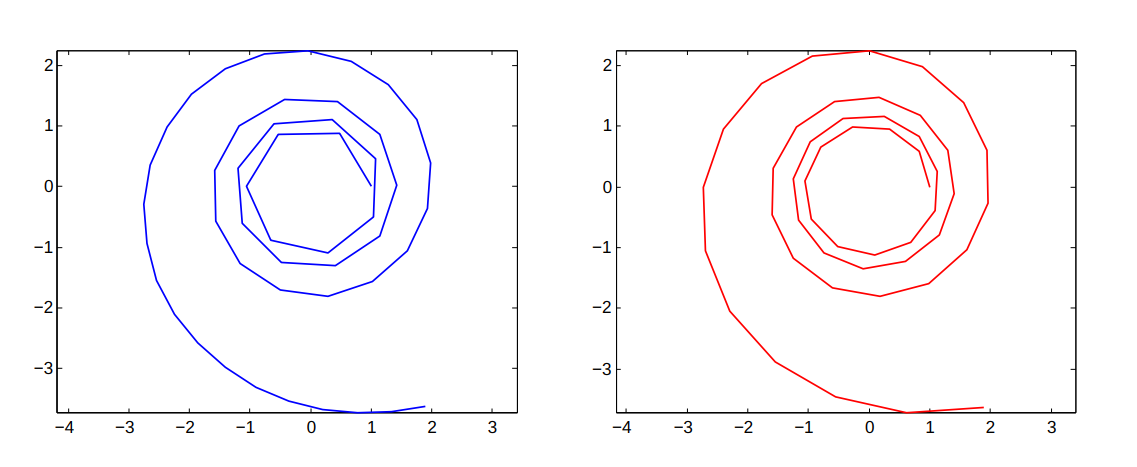
\includegraphics[width=0.9\textwidth]{graphics/sims2.png}
    \caption{
        A trajectory sampled with the same number of (left) time-spaced segments (right) s-spaced segments. Figure retrieved from Yam and Izzo \cite{Yam2010}.
    }
    \label{fig:sundmann_sampling}
\end{figure}

It is evident from Figure \ref{fig:sundmann_sampling} that sampling the $s$ domain is superior in generating a smooth trajectory, in the context of orbital trajectory discretization. This presents an interesting aspect when one considers replacing the temporal variable of time with the s-domain in the context of an infinite-horizon reinforcement learning problem. It would follow that decisions are made more frequently in the vicinity of the singularities, which is desirable for collision avoidance in the context of asteroid exploration, whereas decisions are less frequent further away from the singularities.

%%%%%%%%%%%%%%%%%%%%%%%%%%%%%%%%%%%%%%%%%%%%%%%%%%%%%%%%%%%%%%%%%%%%%%%%%%%%%%%%
\subsection{Satellite Collision Probability}\label{ssec:collision_probability}
%%%%%%%%%%%%%%%%%%%%%%%%%%%%%%%%%%%%%%%%%%%%%%%%%%%%%%%%%%%%%%%%%%%%%%%%%%%%%%%%

Patera \cite{Patera2001} discusses a general method for calculating satellite collision probability which does not make any simplifying assumptions. The process reduces the two-dimensional integral to a one-dimensional integral involving only a simple exponential function in the integrand. This computational efficiency is particularly advantageous when large numbers of collision probability evaluations are performed. The ability to handle asymmetric space objects is beneficial in computing collision probabilities of geostationary satellites with large rectangular solar panels. In many cases, it is possible to mitigate collision risk by reorientating an entire satellite or its appendages. This manoeuvre is far less risky than performing a collision avoidance manoeuvre. Patera provides an accurate and efficient method to calculate orbital collision probability. Their method begins with the three-dimensional Gaussian which describes the uncertainty in the relative position between two objects:

\begin{equation}
    \begin{aligned}
        \rho(\boldsymbol{x}) & =\left[1 /(2 \pi)^{\frac{3}{2}} \sigma_{x} \sigma_{y} \sigma_{z}\right] \exp \left[-\left(x^{2} / 2 \sigma_{x}^{2}\right)-\left(y^{2} / 2 \sigma_{y}^{2}\right)-\left(z^{2} / 2 \sigma_{z}^{2}\right)\right],
    \end{aligned}
    \label{eq:collision_3d_gaussian}
\end{equation}

The original frame defining the density of the relative position uncertainty (\autoref{eq:collision_3d_gaussian}) is related to the encounter frame through the transformation:

\begin{equation}
    \boldsymbol{x}_{\text {sigma}}=U \boldsymbol{x}_{\text {encounter}},
\end{equation}

where $U$ is the transformation matrix. The uncertainty in the original position is then transformed to the two-dimensional encounter frame, providing the two-dimensional Gaussian:

\begin{equation}
    h(\boldsymbol{x})=\left(1 / 2^{\frac{3}{2}} \pi \sigma_{x} \sigma_{y} \sigma_{z} \sqrt{a}\right) \exp \left[-e x^{2}-f y^{2}-g x y\right],
    \label{eq:collision_2d_gaussian}
\end{equation}

where parameters $a, e, f$, and $g$ in \autoref{eq:collision_2d_gaussian} are defined by:

\begin{equation}
    \begin{aligned}
        a & =\frac{U_{13}^{2}}{2 \sigma_{x}^{2}}+\frac{U_{23}^{2}}{2 \sigma_{y}^{2}}+\frac{U_{33}^{2}}{2 \sigma_{z}^{2}}                     \\
        e & =\frac{U_{11}^{2}}{2 \sigma_{x}^{2}}+\frac{U_{21}^{2}}{2 \sigma_{y}^{2}}+\frac{U_{31}^{2}}{2 \sigma_{z}^{2}}-\frac{c^{2}}{4 a}   \\
        f & =\frac{U_{12}^{2}}{2 \sigma_{x}^{2}}+\frac{U_{22}^{2}}{2 \sigma_{y}^{2}}+\frac{U_{32}^{2}}{2 \sigma_{z}^{2}}-\frac{d^{2}}{4 a}   \\
        g & =\frac{U_{11} U_{12}}{\sigma_{x}^{2}}+\frac{U_{21} U_{22}}{\sigma_{y}^{2}}+\frac{U_{31} U_{32}}{\sigma_{z}^{2}}-\frac{c d}{2 a}.
    \end{aligned}
    \label{eq:collision_2d_gaussian:params1}
\end{equation}

The parameters $c$ and $d$ in \autoref{eq:collision_2d_gaussian:params1} are defined by:

\begin{equation}
    \begin{alignat}{2}
        c & =\frac{U_{11} U_{13}}{\sigma_{x}^{2}}+\frac{U_{21} U_{23}}{\sigma_{y}^{2}}+\frac{U_{31} U_{33}}{\sigma_{z}^{2}} \label{eq:collision_2d_gaussian:c}  \\
        d & =\frac{U_{12} U_{13}}{\sigma_{x}^{2}}+\frac{U_{22} U_{23}}{\sigma_{y}^{2}}+\frac{U_{32} U_{33}}{\sigma_{z}^{2}}. \label{eq:collision_2d_gaussian:d}
    \end{alignat}
\end{equation}


\begin{figure}
    \centering
    \captionsetup{format=hang} % hanging captions
    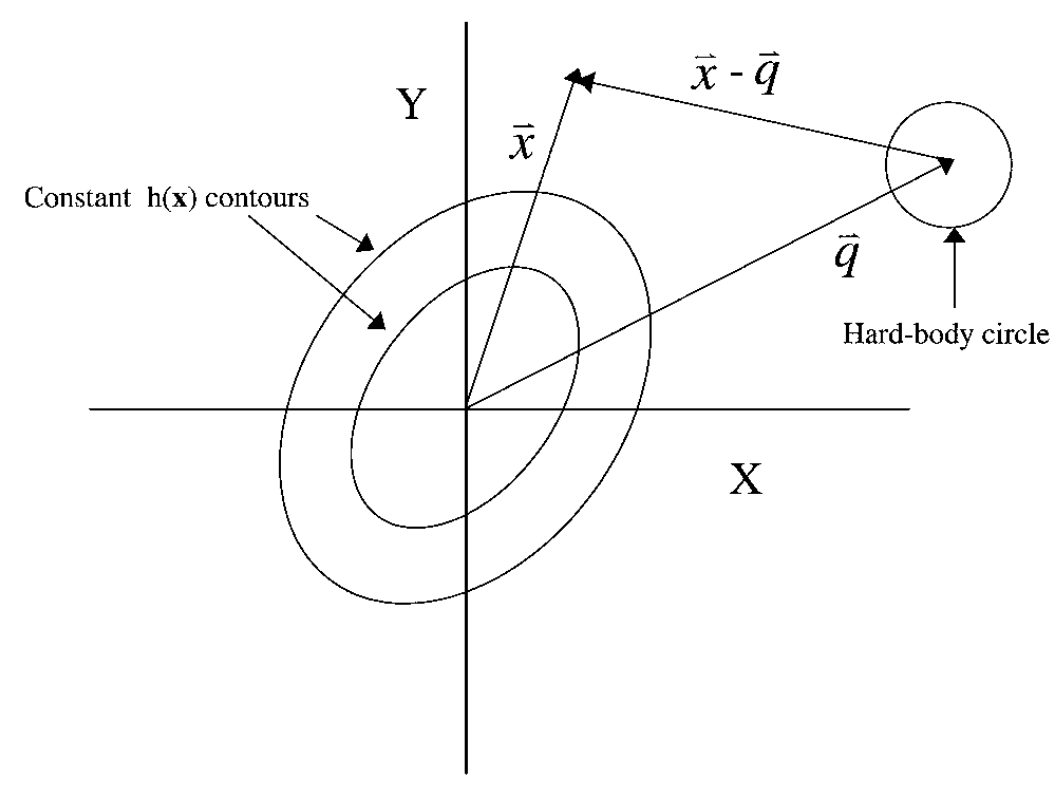
\includegraphics[width=0.5\textwidth]{graphics/encounter-frame.png}
    \caption{\textbf{The two-dimensional Gaussian in the encounter frame}. The uncertainty in relative position between the two objects, denoted by $h(\boldsymbol{x})$. The second object's location $\boldsymbol{q}$ has no uncertainty as all uncertainty is attributed solely to the first object, for visualisation purposes, which is nominally located at the origin. Diagram taken from Patera \cite{Patera2001}.}
    \label{fig:collision_2d_gaussian}
\end{figure}

The second object's location $\boldsymbol{q}$ has no uncertainty as it is attributed solely to the first object, for visualisation purposes, which is nominally located at the origin. For a collision to occur, the actual position of the first object must lie within the hard-body circle for a collision to occur, thus the total collision probability is obtained by integrating $h(\boldsymbol{x})$ over the hard-body circle.

\begin{equation}
    \operatorname{prob}=\iint h(\boldsymbol{x}) u(\boldsymbol{x}-\boldsymbol{q}) \mathrm{d} \boldsymbol{x}
\end{equation}

``A coordinate rotation is performed to eliminate the cross term in $h$ to yield

\begin{equation}
    h(\boldsymbol{x})=\left(1 / 2^{\frac{3}{2}} \pi \sigma_{x} \sigma_{y} \sigma_{z} \sqrt{a}\right) \exp \left[-\alpha x^{2}-\beta y^{2}\right]
\end{equation}

``The correct sign in Eq. (17) is determined by ensuring that the cross term in Eq. (11) is zero, that is,
\begin{equation}
    2(f-e) \sin (\phi) \cos (\phi)+g\left[\cos (\phi)^{2}-\sin (\phi)^{2}\right]=0
\end{equation}

``A scale change in the $y$ axis is made to make $h(x)$ symmetric:''

\begin{equation}
    \begin{gathered}
        y=\sqrt{(\alpha / \beta)} y^{\prime} \\
        h(\boldsymbol{x})=\left(\sqrt{\alpha} / 2^{\frac{3}{2}} \pi \sigma_{x} \sigma_{y} \sigma_{z} \sqrt{a \beta}\right) \exp \left[-\alpha x^{2}-\alpha y^{\prime 2}\right]
    \end{gathered}
\end{equation}

``The $y$ component of $\boldsymbol{q}_{r}, q_{r}(2)$, is multiplied by a scale factor given by

\begin{equation}
    q_{r s}(2)=\sqrt{(\beta / \alpha)} q_{r}(2)
\end{equation}

``The $y$ component of the hard-body circle is also multiplied by the scale factor resulting in


\begin{equation}
    (x / s)^{2}+(y / s)^{2}(\alpha / \beta)=1
\end{equation}

``where $s$ is the initial hard-body radius of the combined objects.

``Using Eq. (20) in Eq. (10) and converting to polar coordinates, one finds

\begin{equation}
    \operatorname{prob}=\frac{\sqrt{\alpha}}{2^{\frac{3}{2}} \pi \sigma_{x} \sigma_{y} \sigma_{z} \sqrt{a \beta}} \iint_{\text {ellipse }} \exp \left(-\alpha r^{2}\right) r \mathrm{~d} r \mathrm{~d} \nu
\end{equation}

``Here the region of integration is defined by the ellipse given by Eq. (22). The advantage of having a symmetric probability density function is now clear because the integration over $r$ can be performed immediately yielding,''


\begin{equation}
    \operatorname{prob}=\frac{1}{4 \sqrt{2} \pi \sigma_{x} \sigma_{y} \sigma_{z} \sqrt{a \beta \alpha}}\left(\int_{s 2} \exp \left(-\alpha r^{2}\right) \mathrm{d} \nu-\int_{s 1} \exp \left(-\alpha r^{2}\right) \mathrm{d} \nu\right)
\end{equation}

``where $s 1$ and $s 2$ are contours defining the hard-body ellipse as shown in Fig. 2. The usual integration technique involves solving for $r$ for each value of $\nu$ along the contours $s 1$ and $s 2$ and determining the endpoints where $s 1$ joins $s 2$. These tedious computations can be avoided by noting that Eq. (24) is equivalent to the closed path integral defined by

\begin{equation}
    \text { prob }=\frac{-1}{4 \sqrt{2} \pi \sigma_{x} \sigma_{y} \sigma_{z} \sqrt{a \beta \alpha}} \oint_{\text {ellipse }} \exp \left(-\alpha r^{2}\right) \mathrm{d} \nu
\end{equation}
% \subsubsection{Analytical Methods}

``where the minus sign is introduced to be consistent with integrating around the contour in the counterclockwisedirection. Equation (25) can be simplified by evaluating the coefficient of the integral, which resultsin Eq. (26a). If the origin is containedin the hard-bodyellipse, the line integral includes an infinitesimal circle about the origin that contributes $a+2 \pi$ to the value of the integral as shown in Fig. 3. In this case Eq. (26a) is replaced with Eq. (26b). When the origin is excluded from the hard-body ellipse,''

\begin{equation}
    \text { prob }=\frac{-1}{2 \pi} \oint_{\text {ellipse }} \exp \left(-\alpha r^{2}\right) \mathrm{d} \nu
\end{equation}

``When the origin is included in the hard-body ellipse,''
\begin{equation}
    \text { prob }=1-\frac{1}{2 \pi} \oint_{\text {ellipse }} \exp \left(-\alpha r^{2}\right) \mathrm{d} \nu
\end{equation}

``The reduction of the probability calculation to a simple contour integral involving only a scalar exponential in the integrand given by Eq. (26) greatly increases computational efficiency. In addition, the ease of defining the closed contour enables the methodology to be applied to the general case of non-sphericalobjects. An example of a non-spherical problem is presented in a subsequent section.''
% \subsubsection{Tracking Methods}
% The orbit determination of an artificial satellite requires empirical observations related to the satellites position of velocity. These observations are collected by a satellites tracking system with the use of electromagnetic wave propagation between a transmitter and a receiver. Each observation corresponding to a unique pair of transmitter and receiver can be generalised as a \textbf{link}.

% % \subsubsection{Radar Tracking}

% % https://solarsystem.nasa.gov/basics/chapter18-1/
% \subsubsection{Deep Space Network (DSN)}

% \cite{Berner2007}

% \begin{itemize}
%     \item \textbf{Frequency \& Timing Data Type, F\&T}
%     \item \textbf{Tracking Data Type, TRK}
%     \item \textbf{Telemetry Data Type, TLM}
%     \item \textbf{Command Data Type, CMD}
%     \item \textbf{Monitor Data Type, MON}
%     \item \textbf{Radio Science Data Type, RS}
%     \item \textbf{Very Long Baseline Interferometry Data Type, VLBI}
% \end{itemize}

% \subsubsection{ESA's tracking station network (Estrack)}


